% ============================================================
%  LOCK_HYBRID_AI - Face & RFID Access Control / Attendance System
%  Edge AI Node (NXP FRDM-MCXN947) + Cloud Backend (FastAPI)
%  Compile: xelatex main.tex  (run twice)
% ============================================================

\documentclass[aspectratio=169, 10pt]{beamer}
\usepackage{fontspec}
% ---- Typography ----
\setmainfont{Inter}
\setsansfont{Inter}
\setmonofont{DejaVu Sans Mono}[Scale=0.85]
\usepackage{beamerthemeBILCS}

% ---- Brand palette, sampled from the school logo (red + deep navy) ----
\definecolor{MLIOTnavy}  {HTML}{16293A}  % deep navy of the globe / book
\definecolor{MLIOTdarkblue}{HTML}{0E1C28}
\definecolor{MLIOTblue}  {HTML}{1E3A52}
\definecolor{MLIOTaccent}{HTML}{B11516}  % logo red
\definecolor{MLIOTaqua}  {HTML}{2F5B7A}
\definecolor{MLIOTgold}  {HTML}{B11516}  % primary emphasis = logo red
\definecolor{MLIOTcoral} {HTML}{8C1114}  % deeper crimson, for alerts
\definecolor{MLIOTlight} {HTML}{E7ECF1}
\definecolor{MLIOTbglight}{HTML}{F4F6F8}
\definecolor{MLIOTfooter}{HTML}{16293A}

% ---- Additional packages ----
\usepackage{amsmath, amssymb}
\usepackage{booktabs}
\usepackage{colortbl}
\usepackage{caption}
\usepackage{hyperref}
\usepackage[loadonly]{enumitem}
\usepackage{array}
\usepackage{pifont}
\usepackage{ragged2e}
\usepackage{fontawesome5}
\usepackage{tikz}
\usepackage[skins]{tcolorbox}
\usetikzlibrary{arrows.meta, positioning, fit, backgrounds, shadows, calc}

\hypersetup{colorlinks=true, urlcolor=MLIOTaccent, linkcolor=MLIOTblue, citecolor=MLIOTblue}

% ---- Assets + accent palette (logo red / navy family) ----
\graphicspath{{assets/}{./}}
\definecolor{LKred} {HTML}{B11516}   % logo red
\definecolor{LKblue}{HTML}{24465F}   % mid navy
\definecolor{LKcyan}{HTML}{2F5B7A}   % light steel blue
\definecolor{LKsky} {HTML}{EEF2F6}   % pale tint (background)
\definecolor{LKink} {HTML}{0E1C28}   % deep ink
\definecolor{LKgreen}{HTML}{1B7A4F}  % "granted" status green
\newcommand{\schoolname}{Blessed International Learning Center Saigon}

% ---- Framed photo helper (white border + soft shadow) ----
\newcommand{\photo}[3][\linewidth]{%
  \begin{tikzpicture}
    \node[inner sep=0pt, line width=1.4pt, draw=white, rounded corners=2.5pt,
          drop shadow={shadow xshift=1.4pt, shadow yshift=-1.4pt, opacity=0.35, fill=black}]
      {\includegraphics[width=#1, height=#2, keepaspectratio]{#3}};
  \end{tikzpicture}}

% ============================================================
%  DESIGN SYSTEM (cards, chips)
% ============================================================
\newtcolorbox{card}[2][]{enhanced, colback=MLIOTwhite, colframe=MLIOTnavy!22,
  boxrule=0.6pt, arc=2mm, boxsep=0.5mm, left=5pt, right=5pt, top=2.5pt, bottom=3pt,
  toptitle=2pt, bottomtitle=2pt,
  fonttitle=\footnotesize\bfseries, coltitle=MLIOTwhite, colbacktitle=MLIOTnavy,
  drop fuzzy shadow={black!35}, title={#2}, #1}

\newtcolorbox{goldcard}[2][]{enhanced, colback=MLIOTwhite, colframe=MLIOTgold!65,
  boxrule=0.6pt, arc=2mm, boxsep=0.5mm, left=5pt, right=5pt, top=2.5pt, bottom=3pt,
  toptitle=2pt, bottomtitle=2pt,
  fonttitle=\footnotesize\bfseries, coltitle=MLIOTwhite, colbacktitle=MLIOTgold,
  drop fuzzy shadow={black!35}, title={#2}, #1}

\newtcolorbox{alertcard}[2][]{enhanced, colback=MLIOTwhite, colframe=MLIOTcoral!55,
  boxrule=0.6pt, arc=2mm, boxsep=0.5mm, left=5pt, right=5pt, top=2.5pt, bottom=3pt,
  toptitle=2pt, bottomtitle=2pt,
  fonttitle=\footnotesize\bfseries, coltitle=MLIOTwhite, colbacktitle=MLIOTcoral,
  drop fuzzy shadow={black!35}, title={#2}, #1}

% ---- Full-width "one line to remember" bars ----
\newtcolorbox{keybar}[1][]{enhanced, width=0.94\textwidth, colback=MLIOTgold!14,
  colframe=MLIOTgold!60, boxrule=0.7pt, arc=2mm, boxsep=0pt,
  left=9pt, right=9pt, top=4pt, bottom=4pt, halign=center,
  fontupper=\footnotesize, drop fuzzy shadow={black!25}, #1}

\newtcolorbox{notebar}[1][]{enhanced, width=0.94\textwidth, colback=MLIOTnavy!7,
  colframe=MLIOTnavy!40, boxrule=0.7pt, arc=2mm, boxsep=0pt,
  left=9pt, right=9pt, top=4pt, bottom=4pt, halign=center,
  fontupper=\footnotesize, drop fuzzy shadow={black!25}, #1}

% ---- Chips ----
\newcommand{\chip}[2]{\tikz[baseline=(t.base)]{\node[rounded corners=2.6pt, fill=#1,
  text=MLIOTwhite, font=\tiny\bfseries, inner xsep=5.5pt, inner ysep=2.4pt] (t) {#2};}}
\newcommand{\chipgold}[1]{\tikz[baseline=(t.base)]{\node[rounded corners=2.6pt, fill=MLIOTgold,
  text=MLIOTwhite, font=\tiny\bfseries, inner xsep=5.5pt, inner ysep=2.4pt] (t) {#1};}}

% ---- Reusable TikZ styles ----
\tikzset{
  lbl/.style={font=\scriptsize\bfseries, MLIOTnavy},
  arr/.style={-{Latex[length=2.6mm, width=1.9mm]}, line width=1.1pt, MLIOTnavy},
}

\newcommand{\thead}[1]{\textcolor{MLIOTwhite}{\textbf{\footnotesize #1}}}

% ============================================================
%  Background, header ribbon, footer
% ============================================================
\setbeamertemplate{background}{%
  \begin{tikzpicture}[remember picture, overlay]
    \shade[top color=white, bottom color=LKsky] (current page.north west) rectangle (current page.south east);
    \fill[LKcyan, opacity=0.06] (current page.south east) -- ++(-3.0,0) -- ++(3.0,3.0) -- cycle;
  \end{tikzpicture}%
}

\setbeamertemplate{frametitle}{%
  \begin{tikzpicture}[remember picture, overlay]
    \fill[MLIOTnavy] (current page.north west) rectangle ([yshift=-0.9cm] current page.north east);
    \shade[left color=LKcyan, right color=MLIOTgold]
      ([yshift=-0.9cm] current page.north west) rectangle ([yshift=-0.95cm] current page.north east);
    \node[anchor=west] at ([xshift=0.42cm, yshift=-0.45cm] current page.north west)
      {
\includegraphics[height=0.56cm]{school_logo.png}};
    \node[anchor=west, text=MLIOTwhite, font=\tiny\bfseries] at ([xshift=1.12cm, yshift=-0.45cm] current page.north west)
      {\schoolname};
    \node[anchor=east, text=MLIOTwhite, font=\scriptsize\bfseries] at ([xshift=-0.42cm, yshift=-0.45cm] current page.north east)
      {LOCK\_HYBRID\_AI};
    \fill[MLIOTgold, rounded corners=1pt]
      ([xshift=0.5cm, yshift=-1.22cm] current page.north west) rectangle
      ([xshift=0.64cm, yshift=-1.62cm] current page.north west);
    \node[anchor=west, text=MLIOTnavy, font=\Large\bfseries, text width=13cm, align=left]
      at ([xshift=0.82cm, yshift=-1.43cm] current page.north west) {\insertframetitle};
  \end{tikzpicture}%
  \vspace{1.34cm}
}

\setbeamertemplate{footline}{%
  \begin{beamercolorbox}[wd=\paperwidth, ht=0.5cm, dp=0.18cm,
        leftskip=0.42cm, rightskip=0.42cm]{footline}%
    \usebeamerfont{footline}%
    \rlap{\textbf{LOCK\_HYBRID\_AI}}%
    \hfill \textit{Face \& RFID Access Control} \hfill
    \llap{\insertframenumber}%
  \end{beamercolorbox}%
}

% ============================================================
%  METADATA
% ============================================================
\title{LOCK\_HYBRID\_AI\\[0.2em]
\large Face and RFID Access Control \& Attendance System}

\author{}

\setAffiliations{%
  Edge AI Node: \textbf{NXP FRDM-MCXN947} \,--\, Cloud Backend: \textbf{FastAPI + SQLite}%
}

\institute{\schoolname}

\date{}

% ============================================================
\begin{document}

% ------------------------------------------------------------
%  TITLE
% ------------------------------------------------------------
\begin{frame}[plain]
  \begin{tikzpicture}[remember picture, overlay]
    \shade[top color=LKink, bottom color=MLIOTnavy]
      (current page.north west) rectangle (current page.south east);
    % ---- school identity ----
    \node[anchor=north] at ([yshift=-0.85cm]current page.north)
      {
\includegraphics[height=2.4cm]{school_logo.png}};
    \node[anchor=north, text=white, font=\scriptsize\bfseries, text width=14cm, align=center]
      at ([yshift=-3.45cm]current page.north) {\schoolname};
    \shade[left color=LKcyan, right color=MLIOTgold]
      ([xshift=-3.6cm, yshift=-4.18cm]current page.north) rectangle
      ([xshift=3.6cm, yshift=-4.23cm]current page.north);
    \node[anchor=north, text=white, font=\fontsize{32}{34}\selectfont\bfseries]
      at ([yshift=-4.55cm]current page.north) {LOCK\_HYBRID\_\textcolor{MLIOTgold!85!white}{AI}};
    \node[anchor=north, text=MLIOTgold!90!white, font=\normalsize\bfseries, text width=13.6cm, align=center]
      at ([yshift=-5.9cm]current page.north) {Face and RFID Access Control \& Attendance System};
    \node[anchor=north, text=LKsky, font=\scriptsize, align=center, text width=14.6cm]
      at ([yshift=-6.75cm]current page.north)
      {Edge AI Node: \textbf{\textcolor{white}{NXP FRDM-MCXN947}} ~~\textcolor{LKcyan}{$\cdot$}~~ Cloud Backend: \textbf{\textcolor{white}{FastAPI + SQLite}}};
    \node[anchor=south, fill=MLIOTgold, text=LKink, rounded corners=3pt, inner xsep=10pt, inner ysep=4pt,
          font=\scriptsize\bfseries] at ([yshift=0.28cm]current page.south)
      {Technical Overview ~~$\cdot$~~ Edge AI on the door, recognition in the cloud};
  \end{tikzpicture}
\end{frame}

% ------------------------------------------------------------
%  1 -- THE PROBLEM AND THE GOAL
% ------------------------------------------------------------
\begin{frame}{The problem, and what the system is for}
  \vspace{-0.1em}
  \begin{card}{\faExclamationTriangle~~Why this system}
    \scriptsize
    \begin{itemize}
      \item Manual attendance is slow and easy to cheat -- one person signs in for another.
      \item A card on its own gets lost, lent out, or cloned -- the UID is not a secret.
      \item Identification must be fast, accurate, and must survive a network outage.
    \end{itemize}
  \end{card}
  \vspace{0.3em}
  \centering
  \renewcommand{\arraystretch}{1.2}
  \scriptsize
  \begin{tabular}{@{}p{3.3cm}p{4.4cm}p{3.6cm}@{}}
    \rowcolor{MLIOTnavy}\thead{Approach} & \thead{Limitation} & \thead{Consequence} \\
    Card only & UID can be cloned (SR-11) & Weak as a sole credential \\
    \rowcolor{MLIOTbglight} Single biometric & Needs contact, slow in a queue & Poor experience at a door \\
  \end{tabular}
  \vspace{0.4em}
  \begin{goldcard}[width=0.92\textwidth]{\faBullseye~~Design goal}
    \scriptsize Combine \textbf{face and card}: unlock in \textbf{under 2\,s} by face or \textbf{under 0.5\,s} by card, keep working offline, and keep the latch \textbf{fail-locked} under every fault.
  \end{goldcard}
\end{frame}

% ------------------------------------------------------------
%  2 -- THE IDEA
% ------------------------------------------------------------
\begin{frame}{LOCK\_HYBRID\_AI in one line}
  \vspace{0.2em}
  \begin{center}
    \begin{goldcard}[width=0.93\textwidth]{\faLightbulb~~Concept}
      \normalsize A system in \textbf{two halves}: the device at the door answers \textit{``is someone there?''}, the server answers \textit{``who is it?''} -- because the processor at the door can find a face, but cannot run the much larger recognition model, and cannot hold the user database.
    \end{goldcard}
  \end{center}
  \vspace{0.55em}
  \begin{columns}[T]
    \begin{column}{0.32\textwidth}
      \begin{card}[halign=flush left]{\faVideo~~Edge Node}
        \scriptsize Detects faces on the integrated NPU, reads RFID cards, drives the door latch.
      \end{card}
    \end{column}
    \begin{column}{0.32\textwidth}
      \begin{card}[halign=flush left]{\faWifi~~Transport}
        \scriptsize ESP32-C5 carries the face image or card UID to the server over Wi-Fi.
      \end{card}
    \end{column}
    \begin{column}{0.32\textwidth}
      \begin{card}[halign=flush left]{\faServer~~Cloud Backend}
        \scriptsize Identifies the face, stores attendance records, serves the admin web app.
      \end{card}
    \end{column}
  \end{columns}
  \vspace{0.5em}
  \centering
  \chip{MLIOTnavy}{Fail-locked by default}\hspace{0.3em}\chip{MLIOTnavy}{Cards work offline}\hspace{0.3em}\chipgold{No face image kept on the device}
\end{frame}

% ------------------------------------------------------------
%  3 -- SYSTEM ARCHITECTURE
% ------------------------------------------------------------
\begin{frame}{System architecture}
  \vspace{0.1em}
  \begin{center}
  \begin{tikzpicture}[font=\scriptsize, scale=0.64, every node/.append style={scale=0.64}]
    \def\py{1.55}\def\pY{-1.55}
    \shade[inner color=MLIOTnavy, outer color=LKink] (-2.7,-0.72) rectangle (0.3,0.72);
    \draw[MLIOTnavy, line width=1pt, rounded corners=6pt] (-2.7,-0.72) rectangle (0.3,0.72);
    \node[text=white, font=\large] at (-1.9,0.34) {\faVideo};
    \node[text=white, font=\normalsize] at (-0.5,0.34) {\faIdCard};
    \node[text=white, font=\footnotesize\bfseries] at (-1.2,-0.16) {Camera + reader};
    \node[text=MLIOTlight, font=\tiny] at (-1.2,-0.48) {OV7670 $\cdot$ MFRC522};

    \def\lx{1.6}\def\lX{5.85}
    \fill[white, rounded corners=6pt] (\lx,\pY) rectangle (\lX,\py);
    \fill[MLIOTnavy, rounded corners=6pt] (\lx,\py-0.68) rectangle (\lX,\py);
    \fill[MLIOTnavy] (\lx,\py-0.68) rectangle (\lX,\py-0.38);
    \draw[MLIOTnavy, line width=1.3pt, rounded corners=6pt] (\lx,\pY) rectangle (\lX,\py);
    \node[text=white, font=\footnotesize\bfseries] at ({(\lx+\lX)/2},\py-0.34) {\faMicrochip~~FRDM-MCXN947};
    \node[anchor=north west, text=MLIOTink, align=left, font=\scriptsize, text width=3.9cm] at (\lx+0.2,\py-0.86)
      {Face \textbf{detection} on the NPU\\[3pt] Device state machine\\[3pt] Drives display + latch};

    \def\mx{6.95}\def\mX{10.75}
    \fill[white, rounded corners=6pt] (\mx,\pY) rectangle (\mX,\py);
    \fill[LKcyan, rounded corners=6pt] (\mx,\py-0.68) rectangle (\mX,\py);
    \fill[LKcyan] (\mx,\py-0.68) rectangle (\mX,\py-0.38);
    \draw[LKcyan, line width=1.3pt, rounded corners=6pt] (\mx,\pY) rectangle (\mX,\py);
    \node[text=MLIOTwhite, font=\footnotesize\bfseries] at ({(\mx+\mX)/2},\py-0.34) {\faWifi~~ESP32-C5};
    \node[anchor=north west, text=MLIOTink, align=left, font=\scriptsize, text width=3.55cm] at (\mx+0.2,\py-0.86)
      {Network transport only\\[3pt] No business logic\\[3pt] SPI to the MCXN947};

    \def\cx{11.9}\def\cX{15.9}
    \fill[white, rounded corners=6pt] (\cx,\pY) rectangle (\cX,\py);
    \fill[MLIOTgold, rounded corners=6pt] (\cx,\py-0.68) rectangle (\cX,\py);
    \fill[MLIOTgold] (\cx,\py-0.68) rectangle (\cX,\py-0.38);
    \draw[MLIOTgold, line width=1.3pt, rounded corners=6pt] (\cx,\pY) rectangle (\cX,\py);
    \node[text=white, font=\footnotesize\bfseries] at ({(\cx+\cX)/2},\py-0.34) {\faServer~~Cloud Backend};
    \node[anchor=north west, text=MLIOTink, align=left, font=\scriptsize, text width=3.75cm] at (\cx+0.2,\py-0.86)
      {API $\cdot$ Recognition Service\\[3pt] Attendance Service\\[3pt] Database $\cdot$ Admin Web};

    \draw[arr, line width=1.5pt] (0.3,0) -- (\lx,0);
    \draw[arr, line width=1.5pt] (\lX,0) -- (\mx,0);
    \draw[arr, line width=1.5pt] (\mX,0) -- (\cx,0);
    \node[text=MLIOTnavy!85, font=\tiny] at ({(\lX+\mx)/2},-0.26) {SPI};
    \node[text=MLIOTnavy!85, font=\tiny] at ({(\mX+\cx)/2},-0.26) {HTTPS};
  \end{tikzpicture}
  \end{center}
  \vspace{0.35em}
  \centering
  \chipgold{\faLightbulb~~Edge: ``is someone there?'' -- Cloud: ``who is it?'' (CON-7, CON-8)}
\end{frame}

% ------------------------------------------------------------
%  4 -- HARDWARE / BILL OF MATERIALS
% ------------------------------------------------------------
\begin{frame}{Hardware and bill of materials}
  \vspace{0.3em}
  \centering
  \renewcommand{\arraystretch}{1.3}
  \scriptsize
  \begin{tabular}{@{}p{4.3cm}p{5.5cm}@{}}
    \rowcolor{MLIOTnavy}\thead{Component} & \thead{Role / Specification} \\
    Controller & NXP FRDM-MCXN947 (integrated NPU) \\
    \rowcolor{MLIOTbglight} Camera & OV7670 (DVP capture via SmartDMA) \\
    RFID reader & MFRC522 (13.56\,MHz) \\
    \rowcolor{MLIOTbglight} Display & 2.4\,inch SPI TFT (240$\times$320) \\
    Latch actuator & Servo motor (defaults to locked -- SR-6) \\
    \rowcolor{MLIOTbglight} Network module & ESP32-C5 DevKit 2.0 (Wi-Fi) \\
    Server & Cloud Backend -- FastAPI + SQLite \\
  \end{tabular}
  \vspace{0.5em}
  \begin{goldcard}[width=0.92\textwidth]{\faCogs~~Hardware design rule}
    \scriptsize Every peripheral connects to the controller and to nothing else -- no peripheral talks to another peripheral directly.
  \end{goldcard}
\end{frame}

% ------------------------------------------------------------
%  5 -- FACE ATTENDANCE FLOW
% ------------------------------------------------------------
\begin{frame}{Flow: attendance by face}
  \vspace{0.3em}
  \begin{center}
  \begin{tikzpicture}[font=\footnotesize]
    \def\dx{3.15}
    \foreach \i in {0,1,2}{
      \pgfmathsetmacro{\xa}{\i*\dx+0.68}
      \pgfmathsetmacro{\xb}{(\i+1)*\dx-0.68}
      \ifnum\i=2
        \draw[-{Latex[length=2.6mm,width=2mm]}, line width=1.6pt, MLIOTcoral!85] (\xa,0) -- (\xb,0);
      \else
        \draw[-{Latex[length=2.6mm,width=2mm]}, line width=1.6pt, MLIOTnavy!35] (\xa,0) -- (\xb,0);
      \fi
    }
    \foreach \i/\col/\ic/\ti/\su in {%
        0/MLIOTnavy/{\faVideo}/{Detect}/{stable for 3 frames},
        1/LKblue/{\faCut}/{Crop \& compress}/{send to the server},
        2/LKcyan/{\faBrain}/{Match}/{compare embeddings},
        3/MLIOTcoral/{\faLockOpen}/{Decide}/{unlock or deny}}{
      \pgfmathsetmacro{\x}{\i*\dx}
      \pgfmathtruncatemacro{\n}{\i+1}
      \fill[\col, opacity=0.14] (\x,0) circle (0.78);
      \shade[inner color=\col!85, outer color=\col] (\x,0) circle (0.6);
      \node[text=white, font=\Large] at (\x,0) {\ic};
      \node[circle, fill=white, draw=\col, line width=0.8pt, text=\col, font=\tiny\bfseries,
            inner sep=0.4pt, minimum size=0.4cm] at (\x+0.48,0.48) {\n};
      \node[text=MLIOTnavy, font=\footnotesize\bfseries] at (\x,-1.02) {\ti};
      \node[text=MLIOTink!75, font=\tiny] at (\x,-1.32) {\su};
    }
  \end{tikzpicture}
  \end{center}
  \vspace{0.45em}
  \begin{columns}[T]
    \begin{column}{0.48\textwidth}
      \begin{goldcard}{\faBolt~~Timing requirement}
        \scriptsize Target \textbf{under 2 seconds} from presenting a face to the latch beginning to open (PR-1). No decision within 5\,s $\rightarrow$ treated as denied (FR-18).
      \end{goldcard}
    \end{column}
    \begin{column}{0.48\textwidth}
      \begin{card}{\faUserShield~~Privacy}
        \scriptsize The captured face is erased from the device as soon as it has been sent -- it is never written to flash or the SD card (SR-3).
      \end{card}
    \end{column}
  \end{columns}
\end{frame}

% ------------------------------------------------------------
%  6 -- CARD FLOW & OFFLINE OPERATION
% ------------------------------------------------------------
\begin{frame}{Cards and offline operation}
  \begin{columns}[T]
    \begin{column}{0.5\textwidth}
      \begin{goldcard}{\faIdCard~~Decided on the device}
        \scriptsize
        \begin{itemize}
          \item The node looks the UID up in its \textbf{local card store}, synchronized from the server -- it does not ask the server on every tap (FR-10a).
          \item Response in \textbf{under 0.5 seconds}, online or offline (PR-2).
        \end{itemize}
      \end{goldcard}
    \end{column}
    \begin{column}{0.5\textwidth}
      \begin{card}{\faWifi~~When the link is down}
        \scriptsize
        \begin{itemize}
          \item Events are \textbf{buffered locally} and carry the time they actually occurred, not the time they were uploaded (FR-20, FR-21).
          \item They are deleted from local storage \textbf{only after the server confirms} each one (FR-22).
        \end{itemize}
      \end{card}
    \end{column}
  \end{columns}
  \vspace{0.6em}
  \centering
  \begin{keybar}
    \faExclamationCircle~~Face access is \textbf{not available} while offline (FR-24) -- only the card path works without a network.
  \end{keybar}
\end{frame}

% ------------------------------------------------------------
%  7 -- DEVICE STATE MACHINE
% ------------------------------------------------------------
\begin{frame}{Device state machine}
  \vspace{-0.15em}
  \begin{center}
  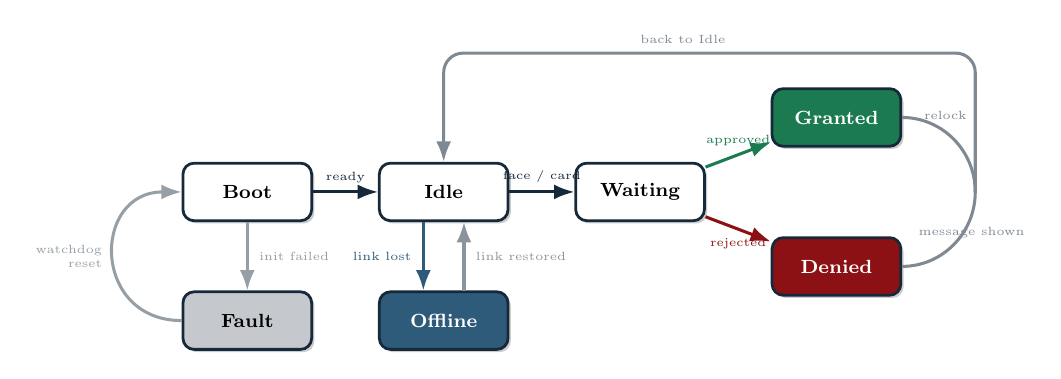
\begin{tikzpicture}[font=\scriptsize, >=Latex, scale=0.86, every node/.append style={scale=0.86}]
    \tikzset{st/.style={draw=MLIOTnavy, line width=1pt, fill=white, rounded corners=4pt,
             minimum width=1.9cm, minimum height=0.85cm, align=center, font=\footnotesize\bfseries,
             drop shadow={shadow xshift=1pt, shadow yshift=-1pt, opacity=0.2, fill=black}}}
    \node[st] (boot) at (0,0) {Boot};
    \node[st] (idle) at (2.9,0) {Idle};
    \node[st] (wait) at (5.8,0) {Waiting};
    \node[st, fill=LKgreen, text=white] (grant) at (8.7,1.1) {Granted};
    \node[st, fill=MLIOTcoral, text=white] (deny) at (8.7,-1.1) {Denied};
    \node[st, fill=LKcyan, text=white] (off) at (2.9,-1.9) {Offline};
    \node[st, fill=MLIOTnavy!25] (fault) at (0,-1.9) {Fault};

    \draw[arr] (boot) -- node[above,font=\tiny]{ready} (idle);
    \draw[arr] (idle) -- node[above,font=\tiny]{face / card} (wait);
    \draw[arr, LKgreen] (wait) -- node[above,font=\tiny]{approved} (grant);
    \draw[arr, MLIOTcoral] (wait) -- node[below,font=\tiny]{rejected} (deny);
    % Boot -> Fault straight down; Fault -> Boot around the left, clear of everything
    \draw[arr, MLIOTnavy!45] (boot.south) -- node[right=1pt,font=\tiny]{init failed} (fault.north);
    \draw[arr, MLIOTnavy!45] (fault.west) to[out=180,in=180,looseness=1.8]
      node[left=1pt,font=\tiny,align=right]{watchdog\\reset} (boot.west);
    % Idle <-> Offline
    \draw[arr, LKcyan] ([xshift=-3mm]idle.south) -- node[left=1pt,font=\tiny]{link lost} ([xshift=-3mm]off.north);
    \draw[arr, MLIOTnavy!50] ([xshift=3mm]off.north) -- node[right=1pt,font=\tiny]{link restored} ([xshift=3mm]idle.south);
    % Granted / Denied merge into one return rail back to Idle
    \draw[MLIOTnavy!55, line width=1.1pt] (grant.east) to[out=0,in=90]
      node[above=1pt,font=\tiny,pos=0.4]{relock} (10.75,0);
    \draw[MLIOTnavy!55, line width=1.1pt] (deny.east) to[out=0,in=-90]
      node[below=1pt,font=\tiny,pos=0.8]{message shown} (10.75,0);
    \draw[arr, MLIOTnavy!55, rounded corners=7pt] (10.75,0) -- (10.75,2.05)
      -- node[above,font=\tiny,pos=0.55]{back to Idle} (2.9,2.05) -- (idle.north);
  \end{tikzpicture}
  \end{center}
  \vspace{0.15em}
  \centering
  \begin{keybar}
    \faLock~~Exactly one state unlocks the latch: \textbf{Granted}. Every other state keeps the door shut.
  \end{keybar}
\end{frame}

% ------------------------------------------------------------
%  8 -- SAFETY & KNOWN LIMITATIONS
% ------------------------------------------------------------
\begin{frame}{Safety and known limitations}
  \begin{columns}[T]
    \begin{column}{0.48\textwidth}
      \begin{card}{\faCheckCircle~~Fail-locked by design (SR-6)}
        \scriptsize The latch returns to \textbf{locked} under every fault: power loss, a software crash, network failure, a peripheral failure, or a corrupt local card store.
      \end{card}
    \end{column}
    \begin{column}{0.48\textwidth}
      \begin{alertcard}{\faExclamationTriangle~~Known limitations}
        \scriptsize
        \begin{itemize}
          \item \textbf{No presentation-attack detection} (SR-7) -- a photograph of an enrolled person may be enough to obtain access.
          \item RFID card UIDs are \textbf{not secret} and can be cloned (SR-11).
        \end{itemize}
      \end{alertcard}
    \end{column}
  \end{columns}
  \vspace{0.6em}
  \centering
  \begin{notebar}
    \faTasks~~Both limitations are stated in the project documentation -- a site that needs protection against them must not rely on face recognition as its sole access control.
  \end{notebar}
\end{frame}

% ------------------------------------------------------------
%  THANK YOU
% ------------------------------------------------------------
\thankyouslide{Full detail lives in \texttt{ARCHITECTURE.md} (design) and \texttt{SYSTEM\_REQUIREMENTS.md} (requirements) of the LOCK\_HYBRID\_AI repository.}

\end{document}
